\section{Практические рекомендации по выбору управляющих структур пневмопривода с дискретными распределителями}

На основе проведенного анализа фронтов Парето были разработаны практические рекомендации
по выбору оптимальных управляющих структур позиционного пневмопривода с дискретными
распределителями в зависимости от типовых предъявляемых требований,
характерных для  конкретных технических задач.

Для наглядного представления предпочтительных областей применения различных
структур управления разработана карта, отображающая эффективность алгоритмов
управления в зависимости от двух ключевых параметров: требуемой точности
позиционирования и ресурсосбережения согласно рисунку~\ref{fig:algorithm_map}.

\begin{figure}[ht]
	\centering
	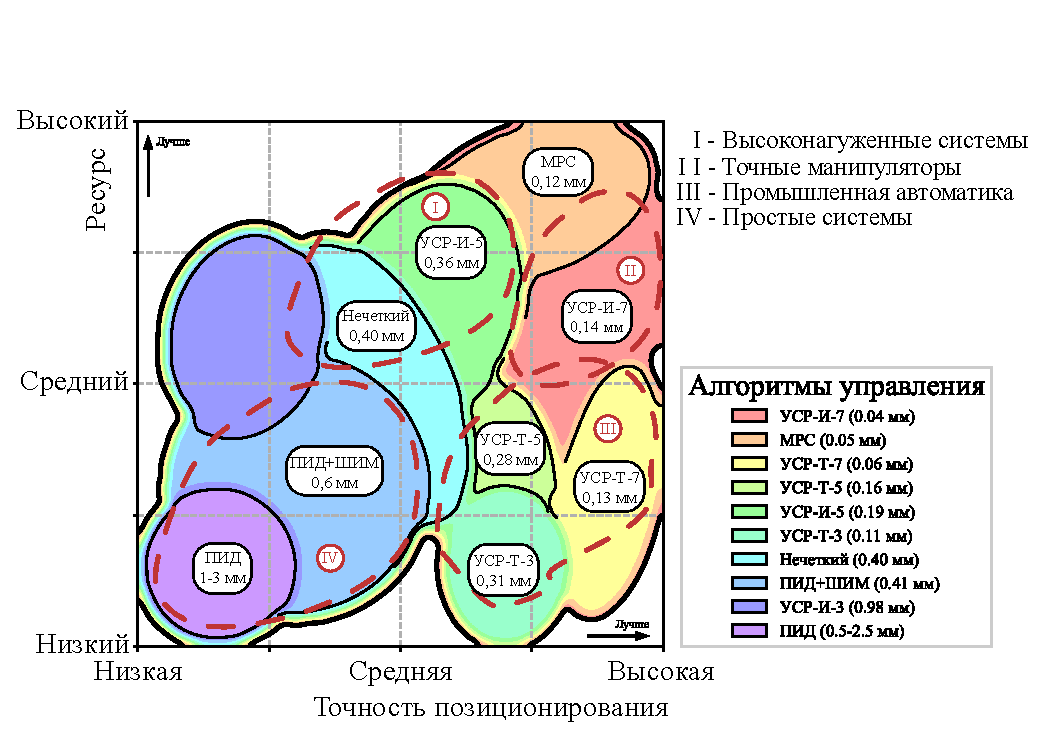
\includegraphics{part5/Карта.eps}
	\caption{Карта предпочтительных областей применения алгоритмов управления:
		горизонтальная ось отражает требуемые динамические качества, вертикальная
		-- ресурсосбережение (минимизацию числа переключений распределителей)}
	\label{fig:algorithm_map}
\end{figure}

На карте предпочтительных областей выделены следующие зоны применения:

\begin{enumerate}
	\item \textbf{Область высоконагруженных систем} (средняя точность позиционирования и
	      высокое ресурсосбережение) -- преимущественная область применения пятирежимного управления
	      в скользящих режимах с интегральной поверхностью (УСР-И-5, 0,36 мм) и прогнозного
	      управления (MPC, 0,12 мм). Эти алгоритмы обеспечивают баланс между точностью
	      позиционирования и высоким ресурсосбережением.

	\item \textbf{Область точных манипуляторов} (высокая точность и высокий ресурс) -- эффективное
	      применение семирежимного управления в скользящих режимах с интегральной поверхностью
	      (УСР-И-7, 0,14 мм), обеспечивающего наивысшую точность позиционирования при сохранении
	      высокого ресурсосбережения.

	\item \textbf{Область промышленной автоматики} (высокая точность и средний ресурс) -- оптимальное
	      использование терминального управления в скользящих режимах (УСР-Т-5, 0,28 мм; УСР-Т-7, 0,13 мм),
	      обеспечивающего хорошую точность позиционирования при средних показателях ресурсосбережения.

	\item \textbf{Область простых систем} (низкая точность и низкие требования к ресурсу) -- рациональное
	      применение ПИД-регулятора (0,5-2,5 мм), ПИД-регулятора с ШИМ (0,6 мм) и трехрежимного управления
	      в скользящих режимах (УСР-И-3, 0,8-1 мм), обеспечивающих невысокую точность позиционирования при
	      низких требованиях к ресурсосбережению.
\end{enumerate}

При выборе алгоритма управления также следует учитывать динамические характеристики
систем через интегральный критерий $ITAE$. Наилучшие показатели по данному критерию
обеспечивают нечеткое управление (0,006 м$\cdot$с²), прогнозное управление (0,012 м$\cdot$с²)
и семирежимное управление в скользящих режимах с интегральной поверхностью (0,019 м$\cdot$с²).

На основе проведенных исследований выработаны конкретные рекомендации по выбору
параметров различных алгоритмов управления для типовых задач позиционирования.
Рекомендуемые значения параметров систематизированы в таблице~\ref{tab:recommended_parameters}.

\begin{table}[ht]
	\centering
	\caption{Рекомендуемые параметры управляющих структур для типовых задач позиционирования}
	\label{tab:recommended_parameters}
	\scriptsize
	\begin{tabular}{p{3.5cm}p{3cm}p{4cm}p{4cm}}
		\midrule
		\textbf{Тип задачи}                                               & \textbf{Рекомендуемая структура} & \textbf{Ключевые параметры} & \textbf{Ожидаемые показатели}   \\
		\midrule
		\multirow{5}{3.5cm}{Прецизионное позиционирование ($AC<0,15$ мм)} & УСР-И-7                          & $\lambda_1=12,5$,           & $AC \approx 0,14$ мм            \\
		                                                                  &                                  & $\lambda_2=0,1$,            & $SI \approx 15$~--~$18$         \\
		                                                                  &                                  & $\varepsilon_1=0,015$,      & $ITAE \approx 0,019$ м$\cdot$с² \\
		                                                                  &                                  & $\varepsilon_2=0,03$,       &                                 \\
		                                                                  &                                  & $\varepsilon_3=0,08$,       &                                 \\
		\hline
		\multirow{5}{3.5cm}{Прецизионное с высоким ресурсом}              & MPC                              & $N_p=15$,                   & $AC \approx 0,12$ мм            \\
		                                                                  &                                  & $N_u=5$,                    & $SI \approx 17$                 \\
		                                                                  &                                  & $Q=100$,                    & $ITAE \approx 0,012$ м$\cdot$с² \\
		                                                                  &                                  & $R=0,1$,                    &                                 \\
		                                                                  &                                  & $\Delta t=0,005$ с          &                                 \\
		\hline
		\multirow{5}{3.5cm}{Промышленные системы}                         & УСР-Т-5                          & $\beta=5$,                  & $AC \approx 0,28$ мм            \\
		                                                                  &                                  & $p=9$,                      & $SI \approx 12$                 \\
		                                                                  &                                  & $q=11$,                     & $ITAE \approx 0,019$ м$\cdot$с² \\
		                                                                  &                                  & $\varepsilon_1=0,025$,      &                                 \\
		                                                                  &                                  & $\varepsilon_2=0,06$        &                                 \\
		\hline
		\multirow{3}{3.5cm}{Системы с повыш. динам. требованиями}         & Нечеткий регулятор               & 5 термов для ошибки,        & $AC \approx 0,40$ мм            \\
		                                                                  &                                  & 5 термов для скорости,      & $SI \approx 27$                 \\
		                                                                  &                                  & 25 правил принятия решений  & $ITAE \approx 0,006$ м$\cdot$с² \\
		\hline
		\multirow{4}{3.5cm}{Высоконагруженные системы}                    & УСР-И-5                          & $\lambda_1=8,5$,            & $AC \approx 0,36$ мм            \\
		                                                                  &                                  & $\lambda_2=0,08$,           & $SI \approx 5$                  \\
		                                                                  &                                  & $\varepsilon_1=0,05$,       & $ITAE \approx 0,033$ м$\cdot$с² \\
		                                                                  &                                  & $\varepsilon_2=0,12$        &                                 \\
		\hline
		\multirow{5}{3.5cm}{Простые системы}                              & ПИД+ШИМ                          & $K_p=4,8$,                  & $AC \approx 0,6$ мм             \\
		                                                                  &                                  & $K_i=0,15$,                 & $SI \approx 34$                 \\
		                                                                  &                                  & $K_d=0,32$,                 & $ITAE \approx 0,021$ м$\cdot$с² \\
		                                                                  &                                  & $f_{ШИМ}=35$ Гц,            &                                 \\
		                                                                  &                                  & $K_т=0,68$                  &                                 \\
		\midrule
	\end{tabular}
\end{table}

Помимо представленных в таблице рекомендаций, необходимо учитывать следующие практические
аспекты при выборе управляющей структуры:

\begin{enumerate}
	\item \textbf{Вычислительная сложность алгоритмов.} Прогнозное управление требует
	      наибольших вычислительных ресурсов и может быть реализовано только на микроконтроллерах
	      с высокой производительностью. Нечеткое управление занимает промежуточное положение по
	      вычислительной сложности. ПИД-регулятор с ШИМ и управление в скользящих режимах могут
	      быть реализованы на микроконтроллерах с ограниченными вычислительными возможностями.

	\item \textbf{Сложность настройки.} ПИД-регулятор с ШИМ имеет наиболее простую процедуру
	      настройки, в то время как прогнозное управление и многорежимное управление в скользящих
	      режимах требуют более тщательной и сложной настройки параметров.

	\item \textbf{Робастность к внешним возмущениям.} Управление в скользящих режимах
	      обеспечивает наибольшую робастность к внешним возмущениям и параметрическим
	      неопределенностям, что особенно важно для систем, работающих в условиях меняющихся нагрузок.

	\item \textbf{Плавность движения.} Нечеткое управление и прогнозное управление
	      обеспечивают наиболее плавное движение привода, что критично для задач, требующих
	      минимизации вибраций и ударных нагрузок.
\end{enumerate}

\subsection*{Методика выбора оптимальной структуры управления}

Для обоснованного выбора оптимальной структуры и параметров позиционного пневмопривода
с дискретными распределителями предлагается методика, представленная в приложении \ref{app:methodology}. Она включает

\begin{enumerate}
	\item \textbf{Анализ требований к системе:}
	      \begin{itemize}
		      \item Определение приоритетных критериев оптимизации (точность позиционирования,
		            быстродействие, ресурс распределителей).
		      \item Установление количественных требований к показателям качества системы.
		      \item Выявление дополнительных ограничений (вычислительные ресурсы, сложность реализации, стоимость).
	      \end{itemize}

	\item \textbf{Предварительный выбор структуры управления:}
	      \begin{itemize}
		      \item Использование карты предпочтительных областей применения для определения
		            подходящих алгоритмов управления.
		      \item Проверка соответствия выбранных алгоритмов дополнительным ограничениям.
	      \end{itemize}

	\item \textbf{Определение параметров выбранной структуры:}
	      \begin{itemize}
		      \item Применение методики решения обратной задачи оптимизации для определения
		            оптимальных параметров.
		      \item Использование рекомендуемых значений параметров из таблицы~\ref{tab:recommended_parameters}
		            в качестве начального приближения.
	      \end{itemize}

	\item \textbf{Верификация выбранной структуры и параметров:}
	      \begin{itemize}
		      \item Проведение моделирования с определенными параметрами.
		      \item Проверка соответствия полученных показателей качества заданным требованиям.
		      \item При необходимости, коррекция параметров или выбор альтернативной структуры.
	      \end{itemize}
\end{enumerate}
